\documentclass[12pt]{report}

\usepackage{graphicx}
\usepackage{tikz}
\usetikzlibrary{shapes.geometric, arrows}
\tikzstyle{startstop} = [rectangle, rounded corners, minimum width=3cm, minimum height=1cm,text centered, draw=black, fill=red!20]
\tikzstyle{process} = [rectangle, minimum width=3cm, minimum height=1cm, text centered, draw=black, fill=blue!20]
\tikzstyle{arrow} = [thick,->,>=stealth]

\begin{document}

\begin{titlepage}
	\centering
    \vspace*{1cm}
	\includegraphics[width=0.3\textwidth]{../images/KMITL Logo.png}

	\vspace{1cm}
	{\LARGE \textbf{Homework 1}} \\[0.5cm]
	\vspace{0.5cm}
	{\large \textbf{Computer Organization and Architecture}} \\[0.5cm]
    {\large \textbf{Software Engineering Program,}} \\[0.5cm]
	{\large \textbf{Department of Computer Engineering,}} \\[0.5cm]
	{\large \textbf{School of Engineering, KMITL}} \\[1cm]
	{\Large 67011352 Theepakorn Phayonrat} \\[0.5cm]
\end{titlepage}

\section*{Topic 1: Linux Booting (Raspberry Pi)}

\subsection*{Question 1: Draw and explain the full boot sequence of Raspberry Pi (from power-on to login).}

\subsection*{Answer:}

When powered on, the Raspberry Pi begins execution from the SoC's built-in boot ROM. The sequence is:
\begin{enumerate}
    \item \textbf{First-stage bootloader} (in SoC ROM) runs on the
        GPU and loads \texttt{bootcode.bin} from the SD card.
    \item \textbf{Second-stage bootloader} \texttt{bootcode.bin}
        initializes SDRAM and loads \texttt{start.elf}.
    \item \textbf{Firmware} \texttt{start.elf} reads configuration
        files (\texttt{config.txt}, \texttt{cmdline.txt}) and loads
        the device tree blob.
    \item It then loads the Linux kernel image (\texttt{kernel.img})
        into memory.
    \item Control passes to the ARM CPU, which executes the kernel.
    \item The kernel initializes hardware, mounts the root filesystem,
        and starts \texttt{systemd}.
    \item \texttt{systemd} launches necessary services and finally
        presents the login prompt.
\end{enumerate}
(Source: https://www.raspberrypi.com/documentation/computers/)

\newpage

\begin{figure}[H]
    \centering
    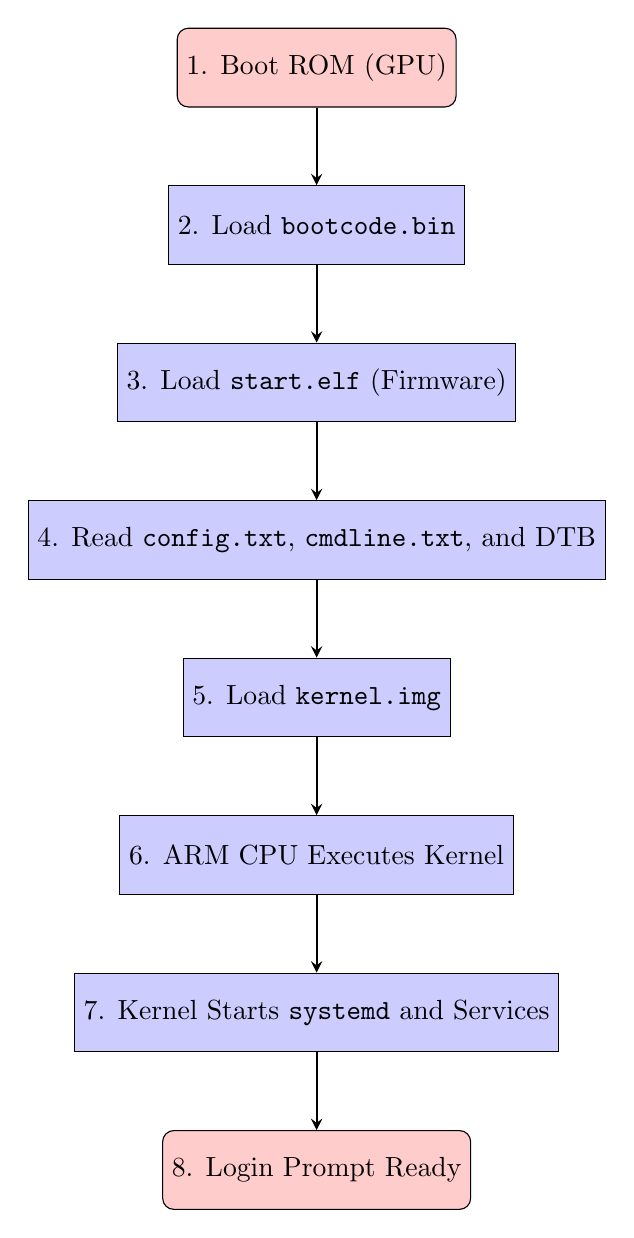
\begin{tikzpicture}[node distance=2cm]
        % Nodes
        \node (rom) [startstop] {1. Boot ROM (GPU)};
        \node (bootcode) [process, below of=rom] {2. Load \texttt{bootcode.bin}};
        \node (firmware) [process, below of=bootcode] {3. Load \texttt{start.elf} (Firmware)};
        \node (config) [process, below of=firmware] {4. Read \texttt{config.txt}, \texttt{cmdline.txt}, and DTB};
        \node (kernel) [process, below of=config] {5. Load \texttt{kernel.img}};
        \node (arm) [process, below of=kernel] {6. ARM CPU Executes Kernel};
        \node (init) [process, below of=arm] {7. Kernel Starts \texttt{systemd} and Services};
        \node (login) [startstop, below of=init] {8. Login Prompt Ready};

        % Arrows
        \draw [arrow] (rom) -- (bootcode);
        \draw [arrow] (bootcode) -- (firmware);
        \draw [arrow] (firmware) -- (config);
        \draw [arrow] (config) -- (kernel);
        \draw [arrow] (kernel) -- (arm);
        \draw [arrow] (arm) -- (init);
        \draw [arrow] (init) -- (login);
    \end{tikzpicture}
    % \caption{Raspberry Pi Boot Sequence Diagram}
\end{figure}

\newpage

\subsection*{Question 2: If the Raspberry Pi fails to boot after update, what steps and files would you check? Explain your troubleshooting process.}

\subsection*{Answer:}

If the Raspberry Pi fails to boot after an update, follow these steps:
\begin{enumerate}
    \item Check the SD card's \texttt{/boot} partition and verify the
        presence of critical files: \texttt{bootcode.bin},
        \texttt{start.elf}, \texttt{kernel.img}, \texttt{config.txt},
        \texttt{cmdline.txt}, and device tree files.
    \item Inspect \texttt{config.txt} and \texttt{cmdline.txt} for
        syntax errors or incorrect parameters.
    \item Attach a serial console to view early boot logs if there is
        no display output.
    \item Test the SD card for corruption; reflash the OS if necessary.
    \item As a final check, boot with a known good SD card to isolate
        hardware issues.
\end{enumerate}
(Source: https://forums.raspberrypi.com/viewtopic.php?t=260328)

\newpage
\section*{Topic 2: BIOS vs UEFI}

\subsection*{Question 1: Create a comparison table (BIOS vs UEFI) and explain why Raspberry Pi doesn't use them and explain why Raspberry Pi doesn't use them.}

\subsection*{Answer:}

\subsection*{Comparison Table}

\renewcommand{\arraystretch}{2} % Increases row height
\begin{tabular}{|X|X|X|}
\hline
\textbf{Feature} & \textbf{BIOS (Legacy)} & \textbf{UEFI} \\
\hline
Firmware Type & Legacy PC-specific code & Modern modular interface \\
\hline
Initialization & Basic hardware init & Rich boot services, network booting \\
\hline
Architecture Support & Primarily x86 & Multi-architecture (x86, ARM, etc.) \\
\hline
Boot Media & MBR only & GPT, large disk support \\
\hline
Extensibility & Minimal & Extensible, supports shell and drivers \\
\hline
\end{tabular}

\subsection*{Why Raspberry Pi Doesn't Use BIOS/UEFI}

Raspberry Pi boots directly using proprietary Broadcom firmware built
into the SoC. This design avoids a separate firmware chip, simplifies hardware, reduces cost, and ensures a lightweight boot process. \\
(Source: https://raspberrypi.stackexchange.com/questions/8475/what-bios-does-raspberry-pi-use)

\newpage

\subsection*{Question 2: If Raspberry Pi adopts UEFI, what would be the pros \& cons?}

\subsection*{Answer:}

\textbf{Pros:}
\begin{itemize}
    \item Standardized boot process.
    \item Support for GPT and large drives.
    \item Easier network booting.
\end{itemize}
\textbf{Cons:}
\begin{itemize}
    \item More complex boot process.
    \item Increased firmware size.
    \item Higher development and maintenance overhead.
\end{itemize}
(Source: https://www.eisfunke.com/posts/2023/uefi-boot-on-raspberry-pi-3.html)

\newpage
\section*{Topic 3: Init and Systemd}

\subsection*{Question 1: Explain how systemd manages a real service (e.g., SSH, Bluetooth).}

\subsection*{Answer:}

For example, the SSH service is managed by \texttt{systemd} using the
unit file \texttt{ssh.service}. To control it:
\begin{verbatim}
sudo systemctl enable ssh     # Enable service on boot
sudo systemctl start ssh      # Start service now
sudo systemctl status ssh     # Check status
sudo journalctl -u ssh        # View logs
\end{verbatim}
Systemd handles dependencies and ensures the service runs in the proper
order during boot. \\
(Source: https://opensource.com/article/20/5/systemd-startup)
\subsection*{Question 2: Map runlevel 5 to systemd target. Show how to change default target via CLI and risks.}

\subsection*{Answer:}

Runlevel 5 (multi-user mode with GUI) maps to \texttt{graphical.target}. To change the default target:
\begin{verbatim}
sudo systemctl set-default graphical.target
\end{verbatim}
To switch immediately:
\begin{verbatim}
sudo systemctl isolate graphical.target
\end{verbatim}
\textbf{Risks:} Using \texttt{isolate} can stop active services
unexpectedly. Changing the default target to \texttt{multi-user.target}
will disable the GUI until changed back. \\
(Source: https://askubuntu.com/questions/788323/how-do-i-change-the-runlevel-on-systemd)

\end{document}
